\documentclass[11pt]{standalone}

\usepackage{helvet}

\usepackage{ifthen}
\usepackage{tikz} 
\usetikzlibrary{shapes.misc}
\usetikzlibrary{arrows,arrows.meta}
\usetikzlibrary{calc,intersections, patterns, math}

\definecolor{pfeil}{RGB}{168,167,167}
\definecolor{petrol}{RGB}{0, 118, 136}
\definecolor{darkgoldenrod}{RGB}{184, 134, 11}
\colorlet{petrol-lighter}{petrol!40}
\colorlet{darkgoldenrod-lighter}{darkgoldenrod!40}

\begin{document}

\def\scl{0.25}

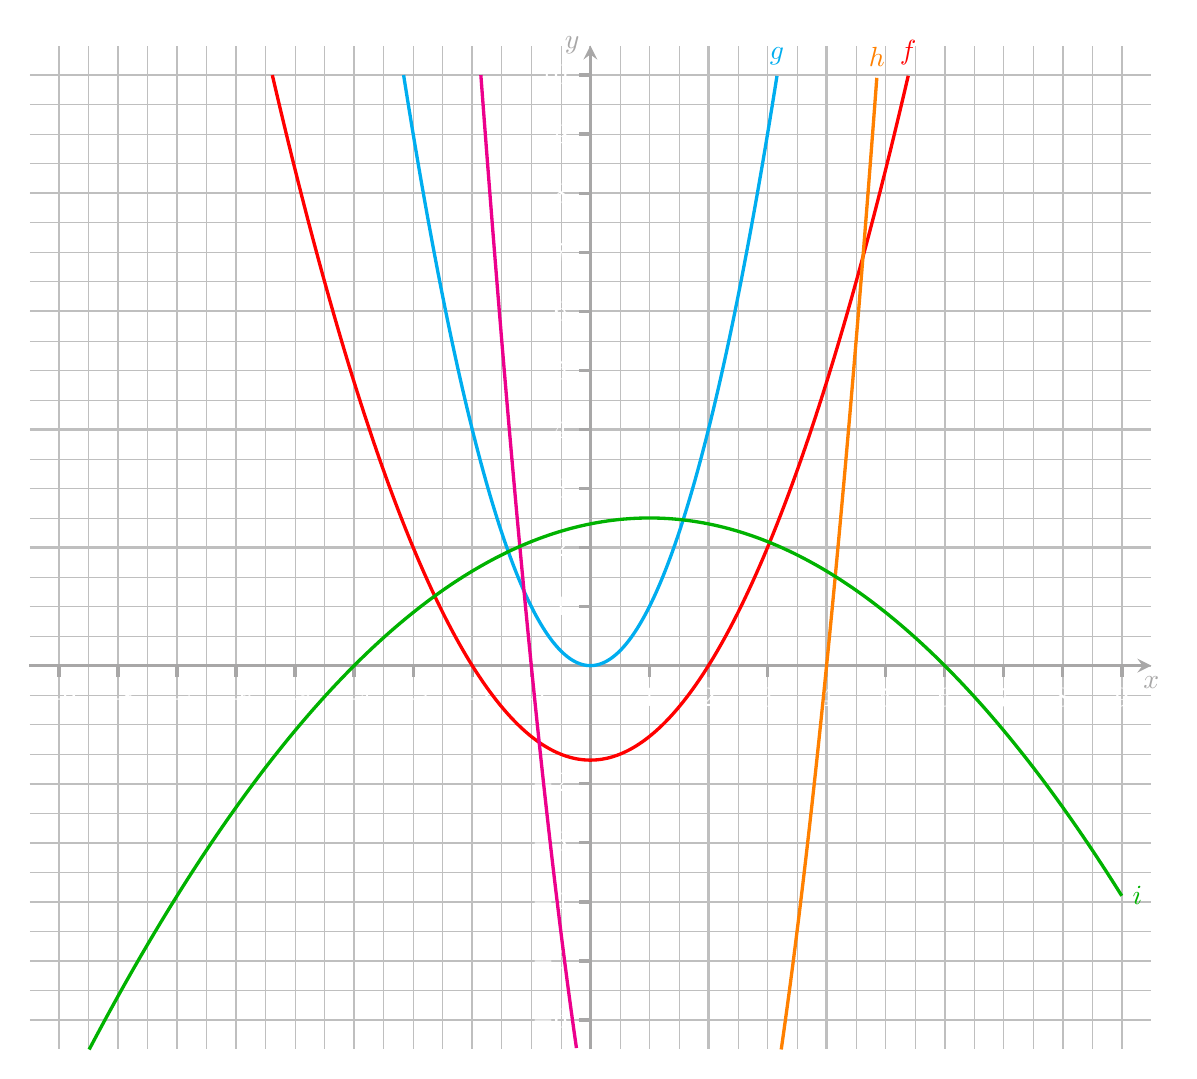
\begin{tikzpicture}[pfeil, scale=0.75,>=stealth] % , scale=\scl

    % \draw[thick, fill=petrol!20, draw=petrol-lighter, rounded corners=2ex, opacity=0.5] (0,0) rectangle ++ (1.5,3.5);
    % \draw[thick, fill=darkgoldenrod!20, draw=darkgoldenrod-lighter, rounded corners=2ex, opacity=0.5] (5,0) rectangle ++ (1.5,3.5);

	\draw[thick, lightgray,step=2] (-9.49,-6.49) grid (9.49,10.49);
	\draw[thin, lightgray,step=1] (-9.49,-6.49) grid (9.49,10.49);
	\draw[very thin, lightgray,step=0.5] (-9.49,-6.49) grid (9.49,10.49);
	%\draw[lightgray,step=0.1] (-9.49,-4.49) grid (9.49,10.49);
	
	\draw[very thick,->] (-9.5,0) -- (9.5,0) node[below]{$x$};
	\draw[very thick,->] (0,-6.5) -- (0,10.5) node[left]{$y$};
	
	\foreach \x in {1,2,...,9}
		\draw[very thick] (\x,0) -- ++ (0,-0.2) node[below, white]{$\x$};
	\foreach \x in {-9,-8,...,-1}
		\draw[very thick] (\x,0) -- ++ (0,-0.2) node[below, white]{$\x$};
	\foreach \y in {1,2,...,10}
		\draw[very thick] (0,\y) -- ++ (-0.2,0) node[left, white]{$\y$};
	\foreach \y in {-6,-5,...,-2}
		\draw[very thick] (0,\y) -- ++ (-0.2,0) node[left, white]{$\y$};
	
	\draw[red, very thick, samples=250, smooth, domain=-5.38516:5.38516]plot (\x,{0.4*(\x+2)*(\x-2)}) node[above]{$f$};
	\draw[cyan, very thick, samples=250, smooth, domain=-3.1623:3.1623]plot (\x,{\x*\x}) node[above]{$g$};
	\draw[magenta, very thick, samples=250, smooth, domain=-1.8541:-0.232051]plot (\x,{2*(\x+1)*(\x-4)});
	\draw[orange, very thick, samples=250, smooth, domain=3.23205:4.8541]plot (\x,{2*(\x+1)*(\x-4)}) node[above]{$h$};
	\draw[green!70!black, very thick, samples=250, smooth, domain=-8.48683:9] plot (\x,{-0.1*(\x+4)*(\x-6)}) node[right]{$i$};

\end{tikzpicture}

\end{document}
